\begin{figure*}[!t]
\centering
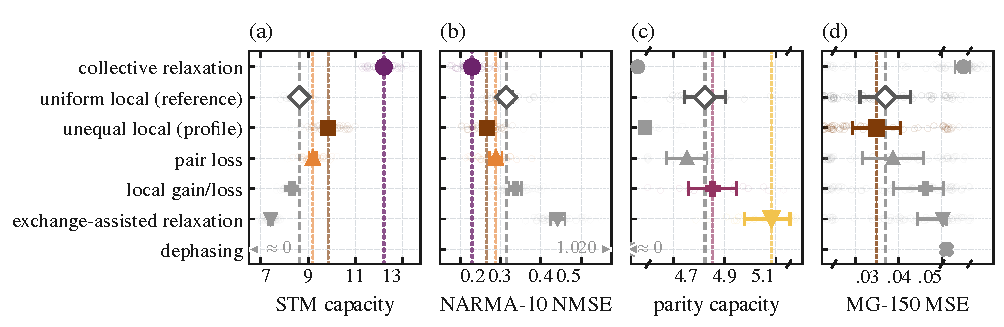
\includegraphics{figures/fig_task_scores.pdf}
\caption{\textbf{Different environmental couplings favor different
computations.}
Scores are shown for continuously driven \(N=5\) reservoirs. Each row
represents one dissipative design. Pale circles show individual reservoirs,
large symbols show the mean, and horizontal bars show pointwise \(95\%\)
intervals. The gray diamond and dashed line mark uniform local relaxation as
the reference. Colored symbols and matching dotted lines identify every design
whose mean outperforms that reference. Higher values are better for STM and
parity, whereas lower values are better for NARMA-10 and MG-150. The broken
axes in (c,d) enlarge the region where the designs differ while retaining all
observations. All designs are compared at the same assigned operator weight
\(\mathcal B\), which provides a common structural reference rather than
physical equivalence. Unequal local differs from the reference only through
its rate profile.}
\label{fig:map}
\end{figure*}

\section{\texorpdfstring{Computational consequences of coupling\\
organization}{Computational consequences of coupling organization}}
\label{sec:performance}

We traverse the two-coordinate design space of Fig.~\ref{fig:space}: first
across jump families, then across rate profiles within a family, and finally
across both axes jointly. We then ask whether exact-expectation differences
remain visible under finite measurement budgets.

\Needspace{6\baselineskip}
The fixed-weight task map establishes task-dependent computation before we
focus on its most strongly replicated consequence: the contrast in
readout-accessible recent-input memory between local and collective relaxation.

\subsection{Reference model and how to read the results}
\label{sec:results-guide}

Uniform local relaxation is the reference, with one equal-rate lowering
channel per qubit. Its family also includes unequal, learned, and
input-adaptive profiles. The main comparison uses the equal-phase rank-one
collective channel with \(c_i=1\) (Appendix~\ref{app:shared}). Profile-optimized
models instead learn within-family coefficients.

The four tasks retain their native metrics: STM and parity capacities are
maximized, whereas NARMA-10 NMSE and MG-150 MSE are minimized.

Figure~\ref{fig:map} reports the absolute \(N=5\) scores in each task's native
metric and favorable direction. The dashed vertical line in each panel marks
the uniform-local mean. Family-colored dotted lines and saturated markers
identify all designs with a better mean in that direction. Faint rings show
individual reservoir instances. The
panels retain their own scales and must be read independently.
Appendix Table~\ref{tab:map} gives the exact means and standard errors.

\subsection{Axis I: Jump-family choice changes the task profile}
\label{sec:map}

We first ask whether changing which system combinations couple to the
environment alters what the reservoir can compute.
\Needspace{5\baselineskip}
Each paired comparison
shares its Hamiltonian, input sequence, operating point, observables, readout,
data split, and structural budget \(\mathcal B\). Only the jump family
changes. Uniform local relaxation supplies the reference, while the
reset-encoded architecture introduced by Fujii and Nakajima (FN)~\cite{Fujii2017} is shown
separately as an external reservoir baseline.

The resulting task profiles differ, and no continuously driven design
dominates all four tasks. Collective relaxation leads STM and NARMA-10 under
the common protocol, but performs worse on parity and long closed-loop
forecasting. Exchange-assisted relaxation provides the clearest parity
improvement.

Under fixed \(\mathcal B\), the map shows protocol-specific specialization, not
a universal winner. A descriptive STM strength sensitivity preserves the
collective lead on the tested grid (Appendix~\ref{app:strength-sensitivity}).
We focus on local versus collective relaxation because it gives the cleanest
comparison within one lowering action and the strongest recurring memory change.

\subsection{Main jump-family case study: collective relaxation versus the
reference model}
\label{sec:collective-case}

We compare complete fixed-budget endpoints with
\(C_{\mathrm{lower}}^{\mathrm{local}}\propto I_N\) and
\(C_{\mathrm{lower}}^{\mathrm{collective}}\propto\boldsymbol c\boldsymbol
c^\dagger\). This endpoint comparison does not identify rank, delocalization,
coefficient-phase pattern, or drive alignment as separately causal.

\begin{figure*}[!t]
\centering
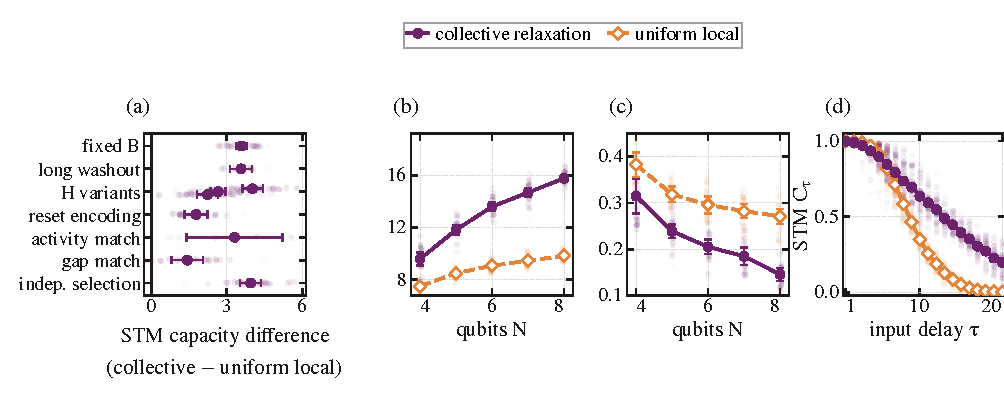
\includegraphics{figures/fig_collective_case.pdf}
\caption{\textbf{Collective relaxation preserves more usable input memory
than uniform local relaxation.}
\emph{(a)} STM gains under the main protocol and targeted controls. Values
above zero favor collective relaxation. \emph{(b,c)} STM capacity and
NARMA-10 error across the tested reservoir sizes. Collective relaxation
retains more memory and gives lower error. \emph{(d)} Memory from each previous
input. The slower purple decline shows that older inputs remain accessible for
longer. Pale marks show individual reservoirs. Large symbols and bars show
means and \(95\%\) intervals.}
\label{fig:collective-case}
\end{figure*}

At \(N=5\), collective relaxation increases STM from \(8.634\) to \(12.206\).
This is an absolute paired gain of \(3.57\) STM-capacity units and a relative
increase of \(41\%\), with a \(95\%\) interval of \([3.36,3.78]\) and \(32/32\)
paired wins. NARMA-10 NMSE decreases from \(0.315\) to \(0.229\), corresponding
to a \(27\%\) reduction in error, and improves in every paired reservoir.

\Needspace{7\baselineskip}
Figure~\ref{fig:collective-case}(b,c) provides a finite-size recurrence check of
the principal \(N=5\) ordering, not an asymptotic scaling analysis. Across 24
paired lineages per size, collective relaxation has the highest mean STM and
the lowest NARMA-10 error from \(N=4\) through \(N=8\).

Before interpreting the larger STM score as useful input memory, we test what
is being remembered. Removing every jump operator while retaining the
Hamiltonian, input protocol, and readout leaves STM and parity near zero,
raises NARMA-10 NMSE above one, and preserves initialization dependence
(Appendix Table~\ref{tab:map}). Coherent driving alone therefore reproduces
neither the task profile nor controlled forgetting. This unmatched diagnostic contrasts
with reset FN, which supplies non-unitary forgetting.

We next distinguish input memory from persistence of the starting state. The
same switched input sequence is applied from four widely separated states, and
their maximum trace distance is tracked. The convergence records in
Appendix~\ref{app:experiment1} show that local relaxation and pair loss
converge across \(N=4,5,6\) and
remain converged through the 1200-input continuation.

\Needspace{3\baselineskip}
Collective relaxation
converges more slowly, but reaches the same regime at the principal \(N=5\)
setting and in the tested \(N=6\) lineages.

\Needspace{4\baselineskip}
At \(N=5\), it approaches numerical
precision by the strict 800-input washout and reaches numerical precision
during the specified continuation to 1200 inputs.

\Needspace{9\baselineskip}
A ten-pair subset of the principal \(N=5\) lineages then uses the 800-input
washout before STM scoring. Cross-initialization differences are negligible,
while collective relaxation retains \(+3.564\,[3.124,4.004]\) STM units with
\(10/10\) wins (Fig.~\ref{fig:collective-case}(a)). For continuous-drive
NARMA-10, all 32 principal pairs are replayed after an independent 600-input
prefix, leaving the scored training and test rows unchanged. At the resulting
800-input washout, NMSE is \(0.315\) locally and \(0.230\) collectively, a
favorable paired difference of \(0.0851\,[0.0716,0.0986]\) with \(32/32\)
wins. The W800-minus-W200 effect change is
\(-0.00007\,[-0.00057,0.00043]\). Across four initial states on the first eight
pairs, the largest W800 NARMA-10 score spread is \(2.18\times10^{-5}\), far
below the smallest paired ground-state improvement, \(0.0148\). The stable
W800 endpoints therefore show that neither ordering is produced by the
residual initial-state dependence exposed at W200.

The comparison is also repeated under four spin-Hamiltonian ensembles that
change the interaction axis, drive axis, interaction form, or connectivity.
Every ensemble retains a positive collective-minus-reference STM difference,
ranging from \(+2.22\) to \(+4.02\) units
(Fig.~\ref{fig:collective-case}(a)). These replications preserve the continuous
encoding and Pauli readout, so they establish recurrence within the tested
driven-spin architecture. Appendix~\ref{app:experiment1} describes the
Hamiltonian variants and ridge control.

To test whether the ordering is tied to continuous-drive encoding, we replace
it with input-by-reset while retaining the \(N=5\) \(XX+Z\) processor, Pauli
readout, task definitions, and fixed structural budget. After an 800-input
washout, collective relaxation increases STM from \(4.596\) to \(6.369\), a
gain of \(1.773\,[1.312,2.235]\), and decreases NARMA-10 NMSE from \(0.673\)
to \(0.491\), a favorable reduction of \(0.182\,[0.144,0.220]\), with \(16/16\)
favorable pairs for both endpoints
(Fig.~\ref{fig:reset-architecture} and
Appendix~\ref{app:reset-architecture}). The ordering between local and
collective relaxation therefore recurs across two tested input architectures rather than being an
artifact of continuous driving.

\subsection{Axis II and joint design: rate profiles refine the chosen
jump family}
\label{sec:profiles}

Choosing a jump family does not fully specify the environmental coupling. A
second choice remains: how should the assigned coupling weight be distributed
within that family? We first keep the local-relaxation family
fixed and compare uniform, random unequal, learned static, and input-adaptive
rate profiles. All sites relax in every candidate, but they need not do so
equally. The profile-only unequal-local row in Appendix
Table~\ref{tab:map} reports the common-protocol comparison. The dedicated STM
sweep below uses the separately
specified profile-optimization protocol.

The uniform profile assigns the same rate to every site. A random unequal
profile introduces a fixed distribution of local timescales. A learned static
profile is fitted separately to each reservoir using validation data. An
adaptive profile varies with the current input. The static profiles share the
same mean rate. The adaptive profile is mean-matched over a fixed input grid
but may vary with the input.

\Needspace{8\baselineskip}
Figure~\ref{fig:profiles}(a) shows that rate redistribution changes STM without
changing the local-relaxation family. Random unequal rates improve on the
uniform-local reference, and reservoir-specific learning improves further.
The learned-minus-uniform gain is \(1.34\) units, with an interval of
\([1.13,1.55]\) and \(32/32\) wins. The adaptive profile gives only a marginal
additional gain under the matched restart and evaluation limits. This ordering
does not establish a general superiority of static profiles because the static
and adaptive parameterizations differ in dimension and stopping behavior.

Within-family tuning redistributes the diagonal rates in the local family,
whereas in the collective family it changes the coefficient vector
\(\boldsymbol c\) and thereby rotates the supported rank-one Kossakowski
direction. Both are well-defined, reproducible tuning operations.

The jump-family and rate-profile axes are not competing alternatives. We therefore
cross them directly by comparing uniform and learned profiles within both
local and collective relaxation at the same \(\mathcal B\).
Figure~\ref{fig:profiles}(b) displays this \(2\times2\) comparison. The vertical
separation shows the jump-family effect, the uniform-to-learned slope shows the
profile effect, and the different slopes show that the profile benefit depends
on the selected family.

\begin{figure}[H]
\centering
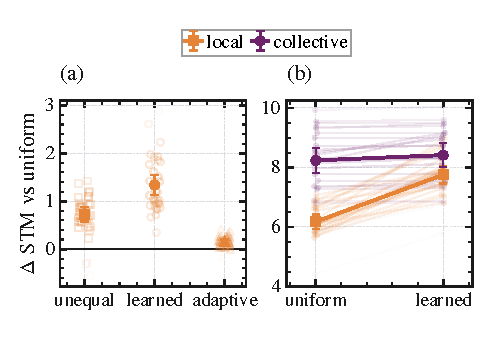
\includegraphics{figures/fig_profiles.pdf}
\caption{\textbf{Rate profiles tune memory within a chosen relaxation
family.}
\emph{(a)} Change in STM relative to uniform local rates for three alternative
profiles. Values above zero indicate improved memory. \emph{(b)} Learning the
rate profile increases STM for both local and collective relaxation, but the
increase is larger for local relaxation. Collective relaxation nevertheless
retains the higher STM overall. Lines connect the same reservoir before and
after learning. Pale marks show individual reservoirs. Large symbols and bars
show means and \(95\%\) intervals.}
\label{fig:profiles}
\end{figure}

The profile gain is larger for local relaxation. The difference between the
two gains is \(1.397\) STM units. All \(24/24\) paired values are positive, and
the familywise \(95\%\) interval is \([1.078,1.716]\). Collective relaxation
nevertheless remains higher after both profiles are learned. Profile
optimization refines the selected family by a family-dependent amount.
Appendix~\ref{app:experiment2} gives the parameterizations and inference scope.

\FloatBarrier
\subsection{Finite sampling determines experimental visibility}
\label{sec:measurement}

The preceding comparisons characterize the computation available to an exact
45-Pauli readout. An experiment observes finite measurement outcomes rather
than exact expectation values. We therefore ask a distinct question: at what
preparation budget do the differences created by coupling organization become
statistically visible?

\FiniteSamplePriorWork

At each step, independent sampling spends \(N_{\mathrm{prep}}=45q\) shots over
45 observables. Grouped sampling spends the same nominal budget in the global
\(X\), \(Y\), and \(Z\) bases and reuses each bitstring across 15 features.
Each design validates its ridge coefficient before one held-out evaluation.
``Preparations per step'' excludes replay of the preceding input history, so
Fig.~\ref{fig:sampling} studies measurement resolution, not end-to-end runtime.

At the exact-expectation endpoint, Fig.~\ref{fig:sampling} recovers the
collective-over-reference memory ordering from the jump-family comparison.
Grouped sampling resolves this contrast with one-sixteenth of the preparation
count needed by independent sampling. This gain is close to the 15-fold
feature reuse built into the estimator. It is a measurement advantage rather
than a hardware advantage specific to collective relaxation.

The finite-data curves also show why measurement design belongs in the
comparison. Sampling noise does not reduce every STM score by the same amount.
At the smallest independent-sampling budgets, pair loss appears best. Unequal
local relaxation leads at intermediate precision. Collective relaxation
emerges only after the observables are estimated accurately enough. Under
simultaneous inference across the complete comparison family, grouped sampling
resolves collective relaxation above every competitor only at the largest
finite budget. Independent sampling never resolves it as best on the tested
grid.

Appendix~\ref{app:experiment3} gives the estimator definitions, budget
parameterization, and simultaneous-inference scope.

\begin{figure}[!t]
\centering
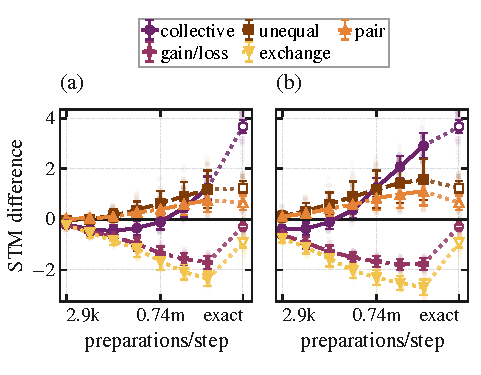
\includegraphics{figures/fig_sampling.pdf}
\caption{\textbf{Grouped measurements reveal memory differences with fewer
preparations.}
Each curve shows the STM difference from uniform local relaxation as the
measurement budget increases. Values above zero indicate more memory than the
reference, and values below zero indicate less. \emph{(a)} Observables are
measured independently. \emph{(b)} Compatible observables are measured
together, making the correct ordering visible with fewer preparations. Open
symbols show the exact results. Pale points show individual reservoir pairs.
Large symbols and bars show means and \(95\%\) intervals.}
\label{fig:sampling}
\end{figure}

Across these analyses, the memory advantage of collective over uniform local
relaxation is the strongest recurring jump-family effect.
Section~\ref{sec:interpretation} now examines which dynamics are consistent
with that contrast.
